\chapter{Compiler Construction}
This chapter will briefly explain the different steps in compiler construction. 
 \begin{figure}[H]
\centering
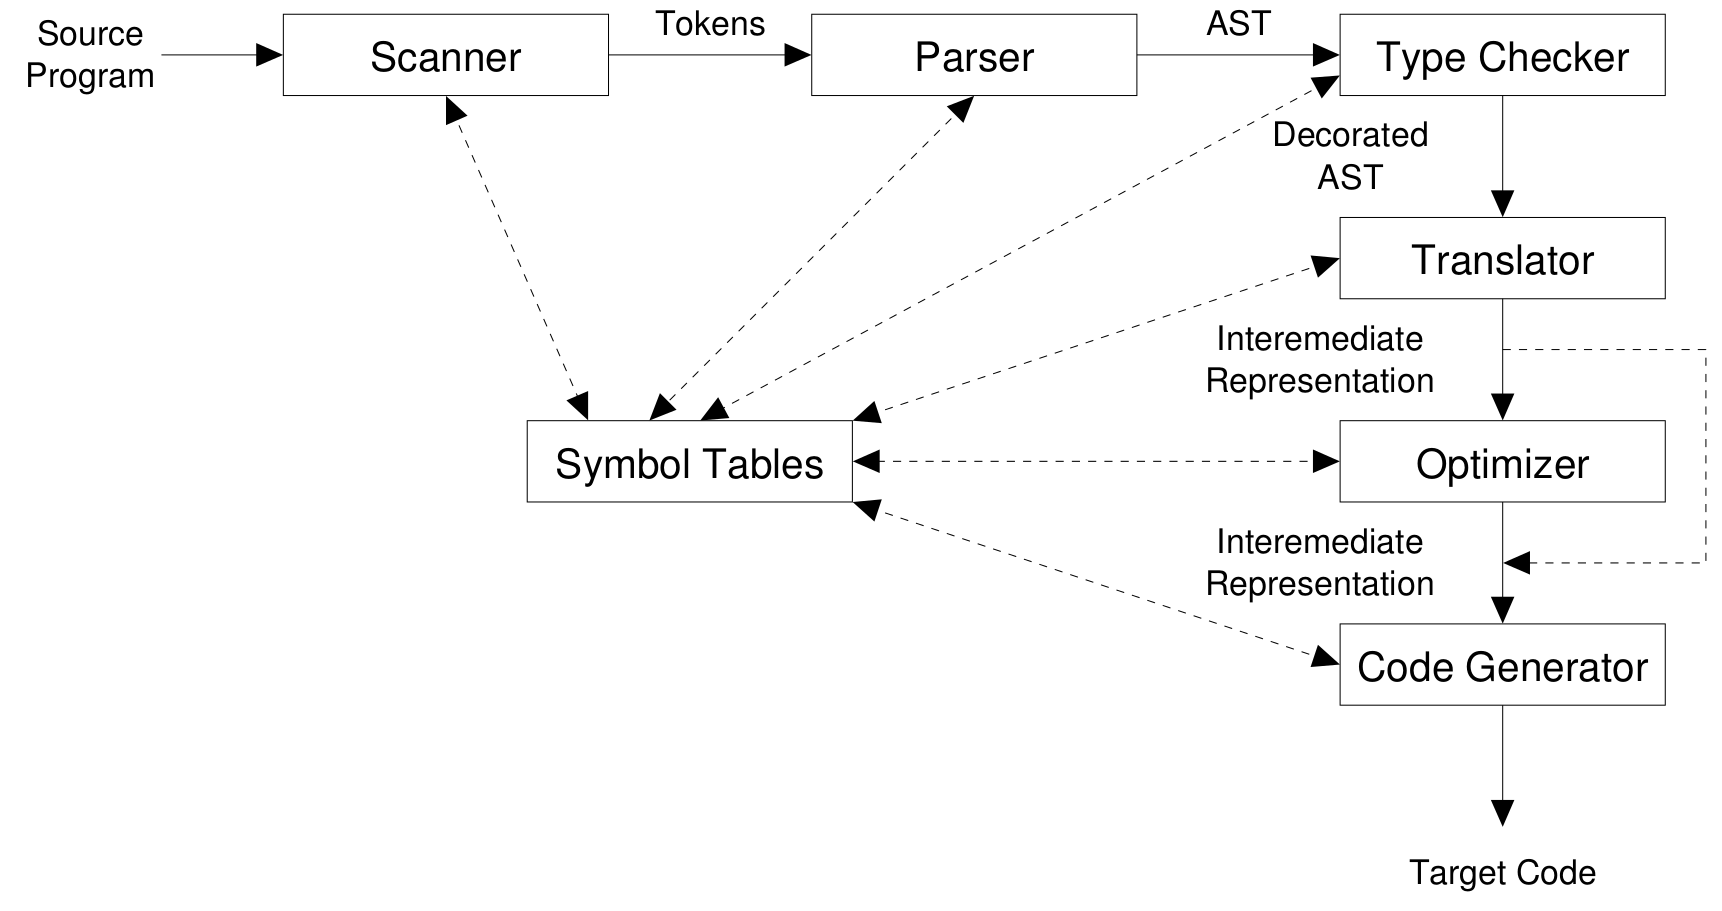
\includegraphics[width=\textwidth]{figures/compiler-process.png}
\caption{Organization of a compiler, Source: Fischer \cite{crafting-a-compiler} }
\label{syntax-overview}
\end{figure}
%This chapter will contain the decisions we made in regards to the compiler of our language, as well as our arguments for making these decisions.

\subsection{The Scanner}
A scanner, also called an Lexer, is the first processing step of a programming language. It reads the input text, ignores comments, and turns it into a compact and uniform format known as tokens. 
A scanner is most often created through declarative programming, meaning to create a scanner you tell a generator what to scan and let the generator do the implementation. What it must scan is specified through regular expressions.

\section{Parsing}
The parser reads tokens generated by the scanner and generates phrases according to a context free grammar file which it then checks are syntactically correct. If there is an error it either reports it, attempts to repair it (to create a syntactically valid program), or tries to recover from the error in order to continue parsing. A parser is typically created through declarative programming. The results of parsing should also be, beside verifying the syntax of an program is valid, to create an abstract syntax tree.

%Parsing is a process where it analyses a string of symbols in a computer language and then trying to understand the meaning of the data that has been constructed. Which can then be made into a parse tree because the parsing understand the relationship by how the string of symbols must be understood. 
%This section will explain on what parsing is, how it works and what kind of different parsing methods exist. 
\\
\subsection*{Top-down and bottom-up parsing}
When constructing a parser, one of two strategies is usually used to recognize and construct tokens based on the context free grammar of the language, namely top-down parsing and bottom-up parsing.\\

Given a starting symbol and a set of rules, a top down parser will start reading its input as a long line of tokens from a lexer. In general, the tokens are read from left to right\footnote{Unless your source language is a language that writes from right to left, of course}, and are afterwards derived from the starting symbol using a leftmost-derivation of the non-terminals through the grammatical rules.

A parse tree represents an ordered structures of data nodes in a hierarchical way, where the nodes above are the parent nodes and the nodes under the parent nodes are the child nodes. It is constructed by a grammer or in this case for the project, a context-free-grammar \\
\begin{figure}[H]
\centering
\frame{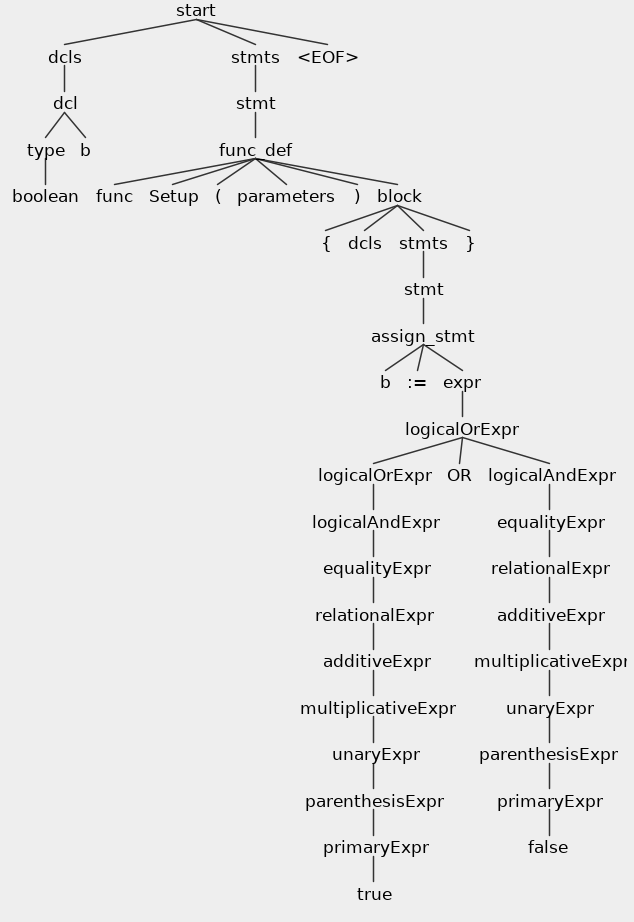
\includegraphics[width=0.7\textwidth]{figures/parse_tree_example.png}}
\caption{}
\label{exampleparse}
\end{figure}
\\
The picture above shows a parse tree, where the highest node, which is A will have 2 child nodes which is B and C. It will than traverse further down until it reaches an end.
The top-down parsing is where the highest node of the parse tree will recognize the detail and from there on go down the parse tree until it hits and recognize the lowest part of the parse tree, which is the most lowest node, but it also reads the leftmost symbol first before going further down. We use top-down parsing when you want to create a hypothetical parsing tree with unknown data relationship, because the parsing tree would be testable to see if the hypothetical unknown data relationship could work together. The top-down parsing uses the LL(1) parsing, which will be explained later\cite{conceptsOfProgrammingLanguages}. 
\\
The buttom-up parsing is where the lowest  part of the parse tree will recognize the smallest part detail first and then go up from there until it hits and recognize the most abstract detail. The buttom-up parsing uses the LR(1) parsing technique unlike the top-down parsing and it scans the right most element first\cite{conceptsOfProgrammingLanguages}. 
\\
\subsection*{LL(k) parsing}
The LL parser (Left to right and left most derivation) is a parser that parses its input from left to right while using a top-down parsing technique. In LL(k) the amount of k is to see how far it has to look ahead.\cite{conceptsOfProgrammingLanguages}

\\
\subsection*{LR(1) parsing}
The LR parser (Left to right and right most derivation) is a parser that parses its input from left to right, but unlike the LL(k) parser, the LR parser uses a buttom-up parsing technique and produces a right most derivation. Just as the LL(k) the the k in the LL(k) defines the amount of tokens the LR will look ahead for\cite{LL-LR-Difference}. 
\\
\subsection*{LALR(1) parsing}
The LALR(k) parser (Look ahead, left to right and right most derivation) is a parser that works the same way as the LR(k) parser, but the difference is that unlike the LR(k) parser the LALR(k) cannot do a backtracking, which is essential an algorithm for the parser to find potential candidates to that maybe can be a solution. If the algorithm finds the potential candidate to be a failure it would go back again to find another potential candidate for the solution. That means that he LALR(k) parser can only look ahead, which makes sense since the parser is by definintion LA(Look ahead)\cite{crafting-a-compiler}.
%Skal have review på LALR siden den forvirre mig. 

\subsection*{Table driven LL(K) parsing}
The table driven LL(k) parser uses a similarity analysis to the genereated grammar so that when it starts with pushing the start symbol into the stack, the parser would try and find match of symbols from the input and when found put the symbol into the top of the stack\cite{crafting-a-compiler}. This is good for when you have a code that is very big and want the parsing to be automatically by using a stack.

\subsection*{Recursive descent parser - not done} 
The recursive descent parser is a top-down parser that is built from a collection of subprograms that each produces its own top-down parse tree generator. The subprograms in itself are recursive and the recursive descent parser will only create one subprogram for every nonterminal it can find in the user generated grammar. \cite{conceptsOfProgrammingLanguages}. 


\subsection{Abstract Syntax Tree}
An abstract syntax tree provides the advantage that 
Removes non essential elements of the syntax. E.g. the colons, equality signs etc. 
Provides a structure which can be altered and annotated to make sure that contextual analysis is performed correctly.
The abstract syntax tree is more an idea since it is very dependent on the construction of the programming language. The idea whole idea is that the entire source program should be stored in the structure and using this structure alone, the compiler programmer should be able to reconstruct the entire source program (Source Bent slides).

\subsection{Type Checker}
During the Type Checker, the types of variables and functions are checked. By saving what the type of each variable is, it is possible to check whether the variables are correctly used. This might be to check if an assignment of the variable is possible or not. This phase is not limited to only type checking. The phase is meant for all the semantic analysis, which is dependant on the compiler programmers. This might include checking for double declaration, declaration before usage, etc.
The result of running the Type Checker is a decorated Abstract Syntax Tree. The abstract syntax tree might is decorated with types but might have other information associated with it, depending on the compiler.

\subsection{Translator}
The translator phase of the compiler takes the decorated abstract syntax tree and makes it into an intermediate representation. The reason for this is that it might be easier to deal with the intermediate representation in the code generation phase.
The translator phase is optional as code can be generated directly from the abstract syntax tree.
The output result is simply the intermediate representation.

\subsection{Optimizer}
The optimizer phase is optional. This is where the code is optimized and bottlenecks are removed. It is done with the idea in mind that you can reduce the size of the code and also reduce the running time of the program. 
\begin{itemize}
    \item Peekhole optimization
    \item Constant folding
    \item Common sub-expression elimination
    \item Code motion
    \item Dead code elimination
\end{itemize}{}

In order to make more efficient code one might eliminate dead variables like this:
\begin{verbatim}
func int magicNumber() {
    int t
    t := 40 * 20 - 100 / 4
    return 42
}
\end{verbatim}
where t is a dead variable.

\subsection{Code Generator}
In the Code Generator phase, the target code is generated. Depending if the compiler generated the intermediate representation or not, the source here is either the intermediate representation or the abstract syntax tree directly. The implementation here is very dependant on the target language as some target languages uses registers directly or stack based machines.

ANTLR4 only provides a context syntax tree (also known as a parse tree) of the source program. The parse tree from ANTLR is the direct translation of the source program parsed by ANTLR using the grammar. The nodes in the parse tree is thus directly related to the tokens provided in the grammar.

To convert the parse tree to a abstract syntax tree, you have to convert every single node to the alternative.
Doing this with ANTLR requires a great overview of both datastructures and the visitor which can be generated by ANTLR. The visitor is an ANTLR specific implementation of the visitor pattern.

\subsection{Visitor pattern}
The visitor pattern is an object oriented pattern provided by the GoF Design Patterns book.
It solves the problem of defining a new operation without changing the classes of the elements on which it operates.
The visitor therefore makes it easy to handler functions for handling the classes in specific contexts. A visitor simply has to specify how to visit all the nodes in the tree.

ANTLR's visitor has generics and implements methods for navigating the entire parse tree both up and down in the tree. That is the way ANTLR has chosen to generate the tree structure.
ANTLR's default BaseVisitor automatically provides an implementation for navigating the parse tree. Thus you only have to override the functionality for the functions where you want to create a node.
As each visit functionality has 2 responsibilities. Generate the node for the abstract syntax tree (with properties) and set the relation between nodes in the node and to it's potential children.
The BaseVisitor also has supports for generics for explicitly tell what should be returned. By simply setting this to a superclass for all nodes in the abstract syntax tree, all functions in the tree should return a node. 

In the end, the object that is returned from the ANTLR BaseVisitor is the top node of the abstract syntax tree.


\subsection{Symboltable}
While the visitor pattern provides a way of handling the nodes in the abstract syntax tree there might be necessary to keep some information when transitioning trough the nodes. This can simply be kept in a private attribute for simple information. However there might be some difficulty dealing when scope rules. Thus it might be nessecary with a symboltable.
A symboltable is datastructure that XX TODO. Whenever opening a new scope the symboltable needs to know and thus declares a new scope. Whenever exiting a scope, close the scope. 
You end up with a decorated abstract syntax tree.

%\subsection{Codegeneration}
%earing the end, of the compiler, after doing all the contextual analysis, you end up with a decorated syntax tree which has made sure that everything lives up to the programming language that has been defined. Now it’s time for code generation.
%Here there can be multiple code generators as it simply can follow the visitor pattern in order to generate the code. This is the point where the designer of the compiler decides what the resulting language of the compiler should be. It could be C, Assembly, etc. It depends on what the programming language is designed for. Sometimes it might be necessary to make some predefined code in order to support the structures and functionality of the programming language.
%A good approach might be to create an intermediate language if you want to compile multiple high-level programming languages to a low-level programming language. In that way instead of making many compilers from D => B, E => B, D => C, E => C, you can simply create one compiler from the high-level language to the intermediate language. Similarly, if you want to output to multiple low level languages, you simply need to add another compiler from the intermediate language to the new low-level language. In that way, instead of making high-level \* low-level number of compilers, you simply have to make Highlevel \+ Low-level number of compilers. It adds abstraction but might also add complexity if either the source language or the destination language has structures which are hard or impossible to implement. Some examples of compilers with intermediate languages are Java and C\#. Java compiles to Java Bytecode which is the instruction set of the Java Virtual Machine. C\# compiles to Common Intermediate Language which is then run on the Common Language Runtime.

\subsection{Compiler}
A compiler is a translator from a source language to a target language.
Depending on the compiler, the compiler may generate one or more of these: Pure Machine Code, Augmented Machine Code or Virtual Machine Code.[Ref Fischer]
In this report the source language is the language "Ezuino" and the target language is Jasmin [TODO].

\subsection{Jasmin}
Jasmin is an assembler for the Java Virtual Machine. It provides takes ASCII syntax of the Java Bytecode and makes into the binary Java Bytecode. [Fischer cap 10.2.2]
